% This file was created by tikzplotlib v0.9.2.
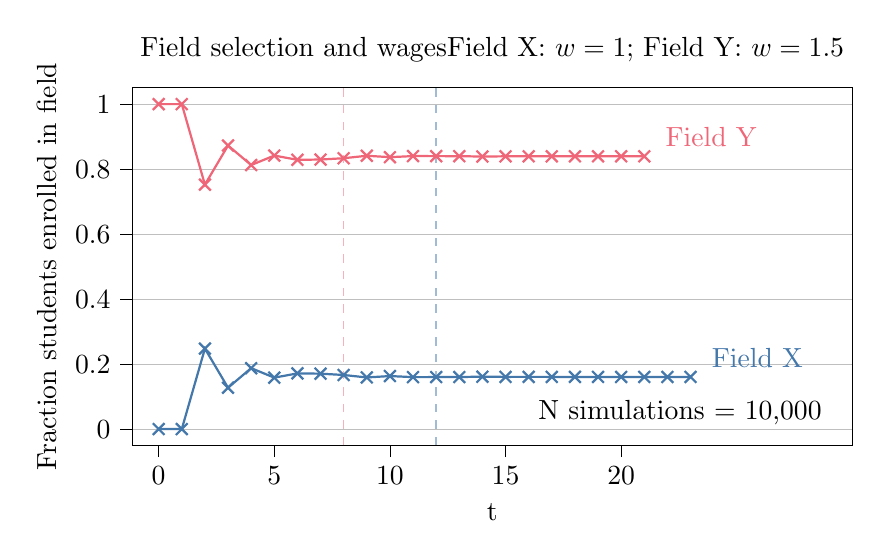
\begin{tikzpicture}

\definecolor{color0}{rgb}{0.266666666666667,0.466666666666667,0.666666666666667}
\definecolor{color1}{rgb}{0.933333333333333,0.4,0.466666666666667}

\begin{axis}[
height=6.121302808757603cm,
tick align=outside,
tick pos=left,
title={Field selection and wages  \\ Field X: \(\displaystyle w = 1\); Field Y: \(\displaystyle w = 1.5\)},
unbounded coords=jump,
width=10.729849cm,
x grid style={white!69.0196078431373!black},
xlabel={t},
xmin=-1.15, xmax=30,
xtick style={color=black},
xtick={0,5,10,15,20},
xticklabels={\(\displaystyle 0\),\(\displaystyle 5\),\(\displaystyle 10\),\(\displaystyle 15\),\(\displaystyle 20\)},
ylabel={Fraction students enrolled in field},
ymajorgrids,
ymin=-0.05, ymax=1.05,
ytick style={color=black},
ytick={0,0.2,0.4,0.6,0.8,1},
yticklabels={\(\displaystyle 0\),\(\displaystyle 0.2\),\(\displaystyle 0.4\),\(\displaystyle 0.6\),\(\displaystyle 0.8\),\(\displaystyle 1\)}
]
\addplot [thick, color0, mark=x, mark size=3, mark options={solid}]
table {%
0 0
1 0
2 0.2477
3 0.1273
4 0.1875
5 0.1583
6 0.1714
7 0.1705
8 0.1665
9 0.1589
10 0.1632
11 0.1599
12 0.16
13 0.1602
14 0.1613
15 0.1606
16 0.1607
17 0.1606
18 0.1606
19 0.1605
20 0.1605
21 0.1605
22 0.1605
23 0.1605
};
\addplot [thick, color1, mark=x, mark size=3, mark options={solid}]
table {%
0 1
1 1
2 0.7523
3 0.8727
4 0.8125
5 0.8417
6 0.8286
7 0.8295
8 0.8335
9 0.8411
10 0.8368
11 0.8401
12 0.84
13 0.8398
14 0.8387
15 0.8394
16 0.8393
17 0.8394
18 0.8394
19 0.8395
20 0.8395
21 0.8395
22 nan
23 nan
};
\addplot [semithick, color0, opacity=0.5, dashed]
table {%
12 -0.05
12 1.05
};
\addplot [semithick, color1, opacity=0.5, dashed]
table {%
8 -0.05
8 1.05
};
\draw (axis cs:23.5,0.1905) node[
  anchor=base west,
  text=color0,
  rotate=0.0
]{Field X};
\draw (axis cs:21.5,0.8695) node[
  anchor=base west,
  text=color1,
  rotate=0.0
]{Field Y};
\draw (axis cs:16,0.03) node[
  anchor=base west,
  text=black,
  rotate=0.0
]{N simulations = 10,000};
\end{axis}

\end{tikzpicture}
